\documentclass[a4paper,11pt]{bxjsarticle}
\usepackage{xltxtra}
\usepackage{zxjatype}
\usepackage{here}
\setjamainfont[BoldFont=ipaexm.ttf]{ipaexm.ttf}
\setjasansfont[BoldFont=ipaexg.ttf]{ipaexg.ttf}
\usepackage{enumitem}
\usepackage{amsmath}
\usepackage{amssymb}
\usepackage{booktabs}
\usepackage{listings}
\usepackage{bm}
\lstset{
basicstyle={\scriptsize}
}
\setlist[enumerate]{listparindent=2pt}


\begin{document}
\begin{titlepage}
  \begin{center}
    \vspace*{150truept}
    {\Huge マルチメディア工学Ⅰ 中間レポート}\\ % タイトル
    \vspace{120truept}
    {\huge 18T1694W}\\ % 学籍番号
    \vspace{50truept}
    {\huge 島袋 隆也}\\ % 著者
    \vspace{50truept}
    {\huge \today}\\ % 提出日
  \end{center}
\end{titlepage}


%=====================================================================
\section{目的}
 本実験では,撮影した画像の圧縮率を変化させ,圧縮による画像劣化を考察する.また,
PNGやGIFに変換し,保存形式による画質の変化を考察し理解することを目的とする.


%=====================================================================
\section{実験器具}
  今回撮影に使用したスマホのスペックを表に示す. 
  \begin{table}[htb]
    \begin{center}
      \caption{スペック表}
      \begin{tabular}{|c|c|} \hline
        名称 & Garaxy s10  \\
        F値 & 2.4  \\
        画素数 & 1200万  \\ \hline

      \end{tabular}
      \label{tab:price}
    \end{center}
  \end{table}

\section{原理}
\subsection{JPEG}
JPEG(Joint Photographic Experts Group)とは,静止画像データを非可逆圧縮する方式の一種である.
この手法は次の2つの処理が行われる.
\begin{enumerate}
  \item 色情報の圧縮
  \item 空間周波数成分分析による圧縮
\end{enumerate}

まず一つ目の色情報の圧縮について説明する.
人の目は輝度と比較し,色の変化には弱い.この特性を利用し,$R$,$G$,$B$の各成分を輝度$Y$と色を表す$C_b$,$C_r$に変換する.
その後,色の成分を平均化し間引くことによってデータが圧縮される.

次に,空間周波数成分分析による圧縮について説明する.
この手法では,元画像の各成分について,8×8画素ごとの小ブロックに分割し,各小ブロックについてDCT演算を行う.
DCTを実際に行った場合を図\ref{fig:dct}に示す.

\begin{figure}[htbp]
  \centering  % 図を真ん中に配置
  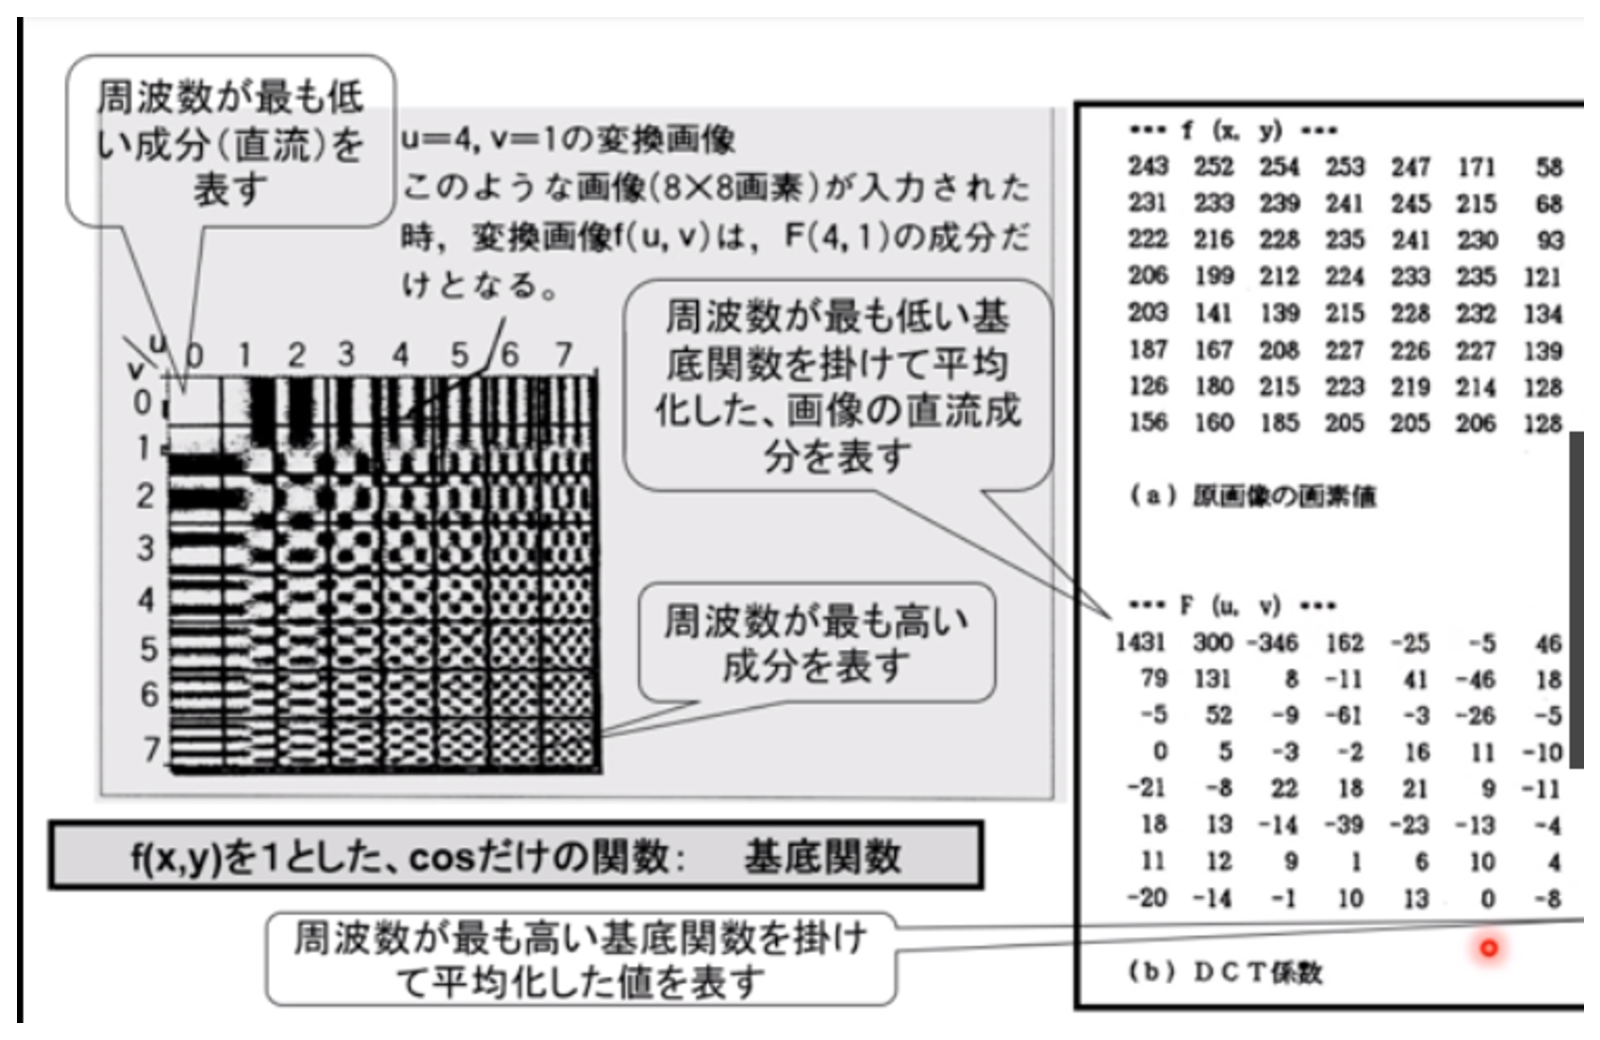
\includegraphics[clip,width = 8.0cm]{dct_con.eps}
  \caption{DCT変換}
  \label{fig:dct}
  \end{figure}

左上の方ほど空間周波数が低く,変化が少ない,その一方で右下の方ほど空間周波数が高い,変化が細かいことが確認できる.
高い空間周波数はデータ量が少ないことから,間引いても違和感なく圧縮できる.

このようにして,圧縮は行われる.

\subsection{PNG}
 
\subsection{GIF}

%=====================================================================
\section{課題}
課題内容を以下に示す.

 \begin{enumerate}
    \item デジカメ等で撮影したJPEG画像の圧縮率を変化させて保存した複数の画像を作成し,画質とデータサイズとの関係を考察しなさい。また,画質がどのように変化しているか。またなぜそのような変化をするのかを考察しなさい。
    \item 同じ画像をJPEG以外の画像フォーマットで保存し,JPEGとの比較考察をしなさい。
  \end{enumerate}



\section{実験手順}
実験器具で示したスマートフォンと画像編集ソフトIrfanViewで実験を行った.
実験手順を以下に示す.\\

\begin{enumerate}
  \item \begin{enumerate}
          \item スマホで写真を撮影する.
          \item IrfanViewで写真を開く.
          \item "ファイル" → "名前をつけて保存"を選択する.
          \item ファイルの種類を"JPG-JPEG File"にする.
          \item "save options"より"save quality"(圧縮率)を0~100の10刻みで実行する.
        \end{enumerate}
  \item \begin{enumerate}
          \item ファイルの種類を"PNG-Portable Network Graphics"にする.
          \item "save options"よりsave quality(圧縮率)を0\textasciitilde100の10刻みで実行する.
          \item ファイルの種類を"GIF-Compuserve GIF"にする.
          \item "save options"よりsave quality(圧縮率)を0\textasciitilde100の10刻みで実行する.
        \end{enumerate}
\end{enumerate}



%=====================================================================
\section{結果と考察}
圧縮率を0\textasciitilde100まで10\%刻みで行った.その結果を図\ref{}から図\ref{}に示す.
  \subsection{結果}
  \begin{enumerate}
    \item 
  \end{enumerate}

   

  \subsection{考察}
  高い圧縮率でJPEG圧縮をすると、8×8で圧縮処理を行う弊害として、以下の画像のように8×8のモザイク状のノイズ(ブロックノイズ)が生じてしまったり、高い空間周波数成分を間引いてしまったために、明るさや色が急激に変わる輪郭周辺でもやもやしたノイズ(モスキートノイズ)が現れたりすることがあります。
   また、圧縮するたびにデータの一部分が必ず劣化していきますので、画像処理を続けて行うときに、途中経過をJPEG形式で保存することはおすすめできません。
   少しでも画像劣化を避けたい場合、あるいは画像処理を続けて行う際の途中経過の保存などのためには、可逆圧縮方式を利用したPNGなどの別の形式を用いるか、データ量は少々多くなりますが圧縮しないでそのまま保存するなどの方法をとることがのぞましいです。


%=====================================================================
\section{参考文献}
マルチメディア工学Ⅰ第六回授業スライド \\


\end{document}
